\documentclass[11pt,twoside,a4paper]{report}
\usepackage[utf8]{inputenc}
\usepackage{amsmath}
\usepackage{amsfonts}
\usepackage{amssymb}
\usepackage{url}
\usepackage{graphicx}
\usepackage{caption}
\usepackage{subcaption}
\begin{document}

\title{Evaluation of algorithms for complex shielding in point kernel dose calculations}
\author{Tom Robert Bryntesen}
\date{May 2015}
\maketitle

\begin{abstract}
This thesis compares algorithms for finding the intersections with complex shields as part of the point-kernel algorithm. The calculations is used to visualise radiation in real time which require the calculations of a large number of measurements. The shielding calculations is the most time consuming part of the calculation when there is a complex environment. Three algorithms for calculating shielding have been implemented. One uses boolean operations on primitive shapes like boxes, cylinders and spheres to create complex objects. The second uses a triangulated geometry. The third uses a 3D voxel grid. Each algorithm have been analysed and benchmarked for performance, accuracy and memory usage. The boolean method is the fastest. For the two others there are a tradeoff between accuracy and performance. However both have similar performance when setup to give the same accuracy.

\end{abstract}

\section{Acknowledgements}
I wish to thank my thesis supervisors Lars Magnusson at Østfold University College.

Ife

John Eidar Simensen

...

\tableofcontents

\chapter{Introduction}
In the nuclear field the workers are exposed to the risk of being exposed to radiation. In radiation protected the ALARA principle states that the risk shall be As Low As Reasonably Achievable. 

One way to lower the risk is to teach the workers about radiation. Software that visualise the radiation is helpful in that it lets the user see the radiation. Doing so can help teach about the factors in dose uptake. That is time of exposure, distance and shielding. When preparing for a job the worker can be briefed about the procedure by showing an animation with radiation visualisation. [TODO: ref Iztvan paper].  It is also possible to train on the procedure actively, in an interactive virtual reality environment. By seeing the areas with higher radiation levels the worker can take steps to avoid these, or minimise the time spent there in order to receive a lover dose. 

Another way to lower the risk is for better planning. Given a planning software that could estimate the doses of workers one could experiment to find the scenario that gives the lowest dose. Either by changing where the workers stand or putting up shielding.

This thesis will focus on improving the algorithm used to calculate dose-rates in real time. Specifically how to improve the performance of calculating the intersections with shields in the environment.


\section{Motivation}
In order to visualise radiation or calculate doses one need to do a great number of calculations. Many visualisation takes a 3 dimensional grid of values as input. If there are 20 cells in each dimension it would require 8000 measurements to generate the visualisation. If the scene is changing, for example when a shield or source is moving, the visualisation has to be updated at interactive rates. 

To calculate the dose of a worker over time one needs to integrate the dose-rate over time. For example the software would calculate the dose-rate for the worker every second and add it all up to get the dose. If the procedure last more than an hour thousands of calculations would be needed for each worker. To keep the software responsive the calculation need to be as fast as possible.

There are different ways to represent a radiological scene. If there are measurements in the area then interpolation can be used to estimate the value at an arbitrary position. However this would not allow for a dynamic scene where one can move sources or shields around. Another way is to define sources and shields and calculate the dose-rates from that. Monte carlo methods simulate photons radiating from the source threw the environment until it reaches the measuring position. This is accurate but very slow. The point-kernel method calculates the dose-rate by taking a single ray from the source to the measuring position and uses formulas and statistical data to estimate the dose-rate. This is not as accurate as monte carlo but is very fast. A more indepth description of the calculation methods is given in chapter 2.

One of the inputs to the point-kernel calculation is the how the ray intersects with the shields between the source and measuring position. This is the most time consuming part of the algorithm for a scene with many shields. By improving the performance of the shields calculation the software will run faster giving a better user experience. [TODO: elaborate on other benifits]

This thesis is written in collaboration with Institute for Energy Technology (IFE). They have implemented a point-kernel calculator that is used in their software. It has support for simple shields like boxes and cylinders. They also support a complex shield that uses a triangulated mesh to represent arbitrary shapes. The evaluation of other ways to represent and calculate complex shield can help IFE improve their calculator.


\section{Research Objectives}
The work in this thesis will find alternative ways to represent complex shields. That is shapes that can be arbitrary and concave. Some of the alternatives will be selected and implemented. The implementations will be evaluated and compared. The following research questions will be focused on during the evaluation process:

How fast is the method
How does the shape influence the speed
How accurate is the method
Are the tradeoffs in the way the method are configured, for example between speed, memory and accuracy
How practical is the method for the developer and end user
What is the overhead, how suitable is the method for representing simple shapes

Speed, memory and accuracy will be measured using quantitative measures from benchmarks. 

\section{Scope and limitations}
The implemented software is intended to be used for benchmarking. It will not be integrated into existing dose calculation software. Doing so would require extra work and is not considered important in order to answer the research questions.

When benchmarking the speed of the algorithms the initialisation of the algorithms are not included in the quantitative data. We will however discuss how the algorithms can be generated efficiently and if it can be pre calculated.

\section{Outline}
Background
Chapter 2 gives an introduction to ionising radiation and methods of calculating doses. How the shield intersections are part of the calculation is explained.  A review of relevant ray tracing algorithms are presented. 
Design
Chapter 3 gives a detailed explanation the design of the shield intersection algorithms and the benchmarking framework. 
Implementation
Chapter 4 gives a detailed description of the implementation of the design described in chapter 3.
Performance Investigation
Chapter 5 shows the results of the benchmarks.
Discussion
Chapter 6 presents the findings from the tests.
Conclusion and Future Research
Chapter 7 gives guidelines on when to use each algorithm, based on the findings from the test. Finally some recommendations for future work are offered.



\chapter{Background / Analysis}

notes:
In “Comprehensive support for nuclear decommissioning based on 3D simulation and advanced user interface technologies.” [4] page 375 it says “The investigations were performed using the Halden Planner (Figure 3) and VRdose (see Section 1) software, both of which are tools that offer real-time calculation (update) of personal and collective dose, dose rates and dose history (dose charts) while allowing the user to dynamically modify work scenarios. This greatly facilitates identifying optimal worker routes, shielding configuration, order of subtasks, and
so forth by enabling suboptimal solutions to be quickly rejected. Furthermore, real-time visualisation of radiation risks (dose) [13,14] aids users in understanding the radiological conditions and, thus in determining the best directions for refining a work scenario during the optimisation process.”. In results: “Our investigations show that dynamic (real-time)
tools that produce reasonably accurate radiological risk estimation can provide vital input information for decision-making, such as to be able to make an informed choice between remote-controlled and manual techniques for a decommissioning task.”

\section{Radiation Theory}
Ionising radiation. Alpha, beta, gamma. Focus on gamma since other can be shielded by clothing, gamma can go threw materials of long distances. Energies.


\section{Usage in computing}
fsa
\subsection{applications}

Halden planner and Sim Editor. Other applications,

\section{Monte Carlo}
[3] explains an monte carlo implementation its methods. Too complex to get into in details. But basicly a large number of particles are simulated from source. The amount and energy reaching the receptor determines the dose.

\section{Point-kernel}
Reference Iztvans paper. Show function and explain part containing shielding.
matter and ways to determine results. TODO: try to find some overview/review paper.

Explain how shielding fits into the point kernel equation and that raytracing can be used to find data data needed.

\section{Raytracing}
Raytracing is used to determine distance travelled through shielding. Different ways to represent 
\subsection{Voxels}
fdsf
\subsection{Triangles}
fasdf
\subsection{Primitives}
fdfs
\subsection{Boolean}
df


\chapter{Method}

The method consist of a big O analysis of creation time, running time, memory consumption. Benchmarking of the algorithms against a set of examples against the same criterias. Also covers methodology used in implementing algorithms.

\section{Design and implementation}
Should we talk about development methodology. Iterative, unit tests, version control etc?

The design and implementation of the algorithms and benchmarking code is presented in Chapter 3 and 4. Given the focus on running time the ray tracing code is optimised for speed. 

\section{How to evaluate algorithms}
Overview, analysis, benchmarking and profiling.

\section{Analysis of algorithms}

%http://en.wikipedia.org/wiki/Computational_complexity_theory
%http://en.wikipedia.org/wiki/Analysis_of_algorithms

Discuss advantages and shortcommings of emperical (measured data) and analysis.

“Empirical evidence (also empirical data, sense experience, empirical knowledge, or the a posteriori) is a source of knowledge acquired by means of observation or experimentation.”

\subsection{Running time}
Big O of algorithm

\subsection{Memory usage}
Discuss data structure

\subsection{Correctness}
Are there anyway to analyse this.

\section{Benchmarking}

\subsection{Measurements}
Measure time used to run the algorithms against a choosen dataset

Measure memory used to create and run aglorithms against datasets.

\subsection{Datasets}
What methodoligy is used in choosing datasets


\subsection{Data Collection}
An automatic benchmarking framework was created to be able to rerun the tests automatically. Benchmarks data set was created to be similar to real world usage. The output of the benchmarks are data that can be easily imported into analysis tools.

\subsection{Data analysis}
The benchmarking framework produces quantitative measurement for running time and correctness. This data will be analysed for comparing the algorithms. The experience from implementing the algorithms will also be reported on.

\section{Could do profiling of the code}
Have to find a method for that


\chapter{Design / Planning and Implementation}
how to design the project in order to answer the research question(s)

This chapter describes the design of algorithm chosen for evaluation and the framework written to benchmark it. What test data to use has a great effect on the results. A description of each and why they were chosen are discussed.
\section{Algorithms}
This sections describes the algorithms and the most important implementation details chosen for comparison. 

\subsection{Closed Mesh}
The closed mesh algorithm determines the intersection with the shield by intersecting the segment against the triangles in a mesh. The algorithm first finds all intersections between an infinite ray starting at the source position in the direction of the measurement position. If the start point is inside or outside the shield is determined by counting the number of intersections. It is inside if there are an odd number and outside if there are an even number of intersections. Then the intersections are iterated in sorted order from the source. Stopping when reaching the measurement positions or when there are no intersections left. Intersections are logged be keeping track of when entering and exiting a triangle.

For the algorithm to work there need to be a way to determine if the source position is inside or outside the shield. This can be done if the mesh is closed, that is creating watertight surface that does not self intersect. One can count the number of intersections using an infinite ray starting from the source position. The ray can go in any direction but using the direction to the measurement positions one can reuse the intersection calculations. If the ray intersects an odd number of times the source position is inside.

\subsection{Bounding Volume Hierarchy Mesh}
The bounding volume hierarchy (BVH) mesh shield is an optimised version of the closed mesh. The difference is that the triangles are put in a bounding volume hierarchy of axis aligned bounding boxes (AABBs). The assumption is that this will perform significantly faster. At least for meshes with many triangles. Although at the expense of initialisation time and possible memory.

\subsection{Boolean Shape}
The boolean shape is build from the primitives shapes and are combined using boolean operations. For this benchmark we have limited the number primitives to boxes, spheres and cylinders. The boolean operations are limited to or and subtract operations. The or operations combines a list of children. The subtract operation subtracts one child from another. A child can be a primitive or another boolean operation.

To find the intersections the tree structure formed by the boolean operations and primitives are traversed. The return value of a node in the tree is a sorted list of intersecting line segments. For the primitives this will be where the line segment entered and exited it. For the or boolean operations this will be all the segments of the children merged so that there is no overlapping segments. For the subtract operation this will be all the segments in the second child removed from the segments of the first child.

The returned segments are represented as two values representing the segment endpoint. Each endpoint is represented by an “t” interpolator value from the source position to the measurement position. This way the boolean operations can be performed on 1 dimensional segments, which simplifies the implementation.

position = sourcePosition + t * (measurementPosition - sourcePosition)

\subsection{Voxel grid}
In the voxel grid each cell represents whether or not it is part of the shield. A fast voxel traversal algorithm [2] is implemented. The details of the algorithm is given in the next chapter.


\section{Benchmarking}

\subsection{framework}
For the voxel implementation an analysis of the relationship between number of divisions and the results was performed. For comparisons with the other algorithms the error data was used to select the lowest division that resulted in an error % lower than 1. For the tube and sphere shapes the lowest subdivision resulting in an error % lower than 1 was selected for comparison.

A benchmarking framework was created to produce the quantitative data. The goal of the framework was to simplify the collection of data and to produce unbiased data. The framework was designed to run all tests without the need of any human interaction. This made it easy to rerun the tests if any changes was made to the algorithms. It also made it easy to run the tests repeatedly and generating more reliable results by basing the data on a larger data set.

The benchmarking framework will have a function that benchmarks a shape against a set of segments:

static BenchmarkOutput doBenchmark(String name, Supplier<ComplexShield> shieldCreator, List<Segment> segments, float[] correctTotals)

The name is used to identify the test and is returned in the BenchmarkOutput. 

The shieldCreator creates a shield. All the data must be created in the Suppler.get() method to be able to measure how much memory the shield uses.

The segments are all the line segments to test against the shield. The different algorithms will be tested against the same set of segments.

The correctTotals array contains what is considered to be the correct result for each segment. This is used to calculate the error the tested shield.

The memory, performance and correctness results are stored in BenchmarkOutput. This is the raw data from the benchmarks. The BenchmarkOutput is gathered, processed and written to a file. The file is imported into an external tool that can generate graphs.

A benchmarking class is created that sets up and performs the benchmarking for all the shapes. For each shape it will create a new set of segments. This is because the size of the shapes may vary and the segments must be adjusted accordingly. It will also implement the shieldCreator for each algorithm as well as calculating the correct results for the shape. 

\subsection{Measure memory used}
To calculate the amount of memory used by a shield we will log the memory used by the Java Virtual Machine (JVM), before and after creating it. This will measure the memory needed to hold the data structures used to represent the shield. We will also log the memory used after running all the calculations. This will uncover any caching performed.

[TODO: less technical]
The java.lang.Runtime class is used to calculate the memory used by the JVM. Runtime.freeMemory() returns the approximate amount of free memory and Runtime.totalMemory() returns the total amount of memory in the JVM. The difference between the two is the amount used, in bytes. This includes the garbage currently held by the garbage collector. So before calculating the memory used the garbage collector is invoked using java.lang.System.gc(). Calling the method “suggests that the Java Virtual Machine expend effort toward recycling unused objects in order to make the memory they currently occupy available for quick reuse”, according to the documentation. The calculated memory used are not necessarily 100% correct and this is taken into consideration when analysing the results. 

\subsection{Running time}
To measure running time the java.lang.System.nanoTime() function is used. It is a high resolution timer provided by the Java Virtual Machine. How the JVM calculates the time is not documented and may vary depending on operating system and hardware. The resolution of the timer was instead measured on the machine performing the benchmarks. This was done by calling nanoTime() in a loop and logging the difference in value when it changed. The resolution calculated was 292 nanoseconds. This was considered to be more than enough for measuring the running time of the shielding calculations.

\subsection{Correctness}
The correctness is included in the benchmarking because the algorithms can not, in some cases, represent the real shape of the shield perfectly. Round shapes have to be approximated by for example triangle or voxel representations. There can also be a tradeoff between correctness on one side and running speed and memory usage on the other. A voxel representation can use more cells to get more correct results at the expense of longer traversal times and higher memory usage. 

To determine the correctness of an algorithm it must be compared to what is considered to be correct. Boolean shields will be used as the correct representation for the shapes benchmarked in this thesis. This is because it is the only algorithm that can represent round shapes like spheres and cylinders correctly. Other types of shapes that are not supported by the boolean implementation will not be used in the benchmarks because of the need of having a correct representation.

The correctness is calculated as the sum of the error for each segment. The error for one segment is the absolute difference between the correct and calculated distance traveled. The error percentage is calculated using the correct sum and the sum or errors.

\subsection{Test Data}
The test data for the benchmark includes a set of shapes and the segments that will be tested against the shapes. The shapes are chosen for different reasons. The shape can be realistic, a shape that can be encountered in a real situation. Or it can be stylised, designed to answer a specific research question or a specific performance situation. The segments are designed to be a realistic example of how it would be used in an application.

\subsubsection{Segments}
The segments used in the benchmark are created to mimic that used in a application that visualise radiation. It will have a set of point sources and a set of measurement positions. A segment is created from each point source to every measurement position.  

The measurement positions will created as a 3 dimensional grid that is slightly larger than the bounding box of the shape. The size of each cell is set to the largest dimension of the grid divided by 30. That will give a grid of approximately 10000 measurement positions, given the axis of the bounding box have about the same length. For the point sources, 10 random points inside the bounding box is used. 

\subsubsection{Tub shape}
\begin{figure}[h]
    \centering
    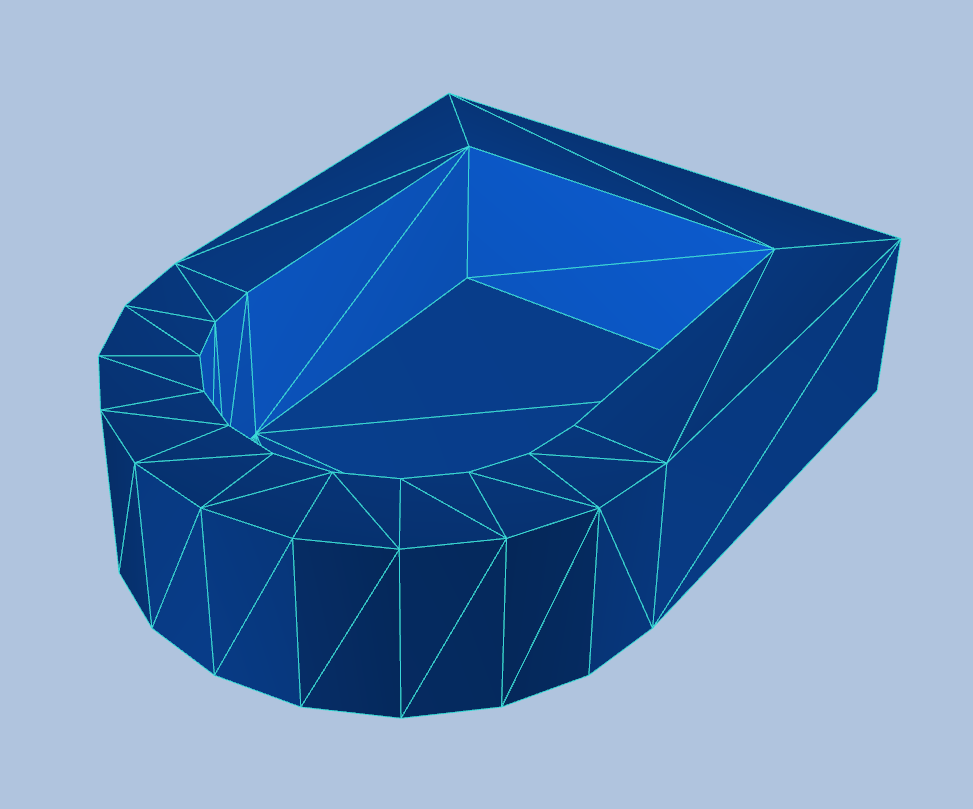
\includegraphics[width=0.45\linewidth]{images/tub_mesh}
    \caption{Tub shape}
    \label{fig:Tub shape}
\end{figure}

The tub shape was chosen because it is a realistic example of a complex shield. A customer of IFE needed to model this shape in the Halden Planner software. At the time there were no support for complex shields. It is one of the concrete reasons why the research into modelling complex shields were started. The shape consist of tub where one side is square and the other is round.

\subsubsection{Building shape}
\begin{figure}[h]
    \centering
    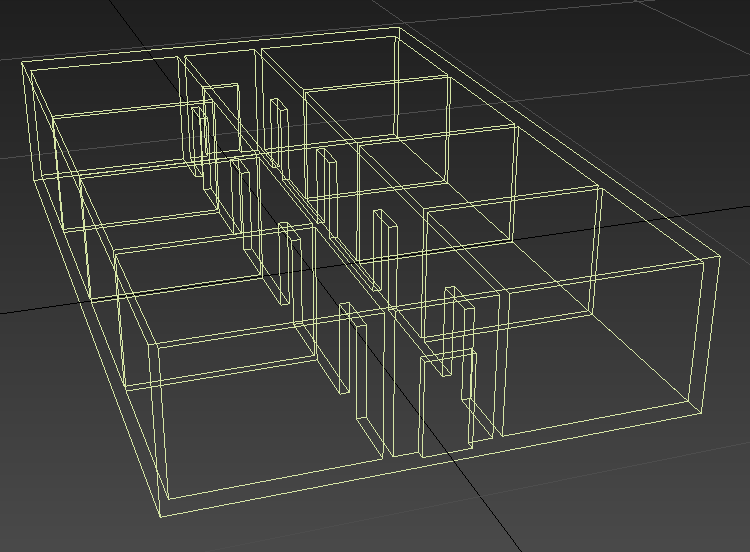
\includegraphics[width=0.45\linewidth]{images/room_max}
    \caption{Building shape}
    \label{fig:Building shape}
\end{figure}
In a radiological scene the building itself can be a major part of the shielding. To test this scenario a floor of a building was modelled. It consist of 8 rooms connected by a hallway. There is a door to each room as well as 2 doors entering the hallway.

\subsubsection{Box shape}
The box shape was included to see how well the complex shields are able to handle simple shapes. The box shape is one of the most useful shapes when building up a realistic radiological scene. If the complex shield handles it well then there might not be need for the application to have specific simple shapes, which can simplify the application. To make the scenario more complex the box is rotated 20, 30 and 40 degrees around the x, y and z axis respectively.

\subsubsection{Sphere shape}
The sphere shape was included to determine how the algorithms manages to represent a round shape. What are the speed, accuracy and memory tradeoffs depending on how tesselated the mesh is or how many cells are used. 

\subsubsection{Tube shape}
\begin{figure}[h]
    \centering
    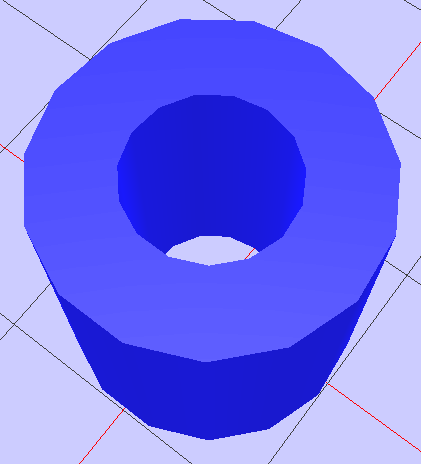
\includegraphics[width=0.45\linewidth]{images/tube_mesh}
    \caption{Tube shape}
    \label{fig:Tube shape}
\end{figure}

The tube shape was included because it is a round shape and it is realistic. There are many shapes in a nuclear power plant that that can be represented by a tube. For example waste containers and pipes.

\chapter{Results}
Outcome of the actual research work described in the implementation.

What can be mentioned: data quality, size of dataset, 

Dimensions: 
-algorithms (mesh, bvh, voxel, bool)
-measures (running time, creation time, memory, correctness)
-analysis methods
  -analysis
  -benchmarking
    -shapes (box, sphere)
    
\section{Correctness}
\subsection{analysis}
\subsection{benchmarking}

\section{Running time}
\subsection{analysis}
\subsection{benchmarking}

\section{Creation time}
\subsection{analysis}
\subsection{benchmarking}

\section{Memory used creating shapes}
\subsection{analysis}
\subsection{benchmarking}
    



\section{Voxel grid}
For the voxel grid the results depends on how coarsely the grid is subdivided. Line graphs are shown to visualise this relationship. The number of division on the longest axis of the shape is used for the x axis. However the grids do not necessarily have the same dimensions on the other axis since the shapes are not square. For example for Axis divisions 200 the grid has the following resolution:
Shape
Grid resolution
Box
199x193x200
Sphere
200x200x200
Tub
200x50x150
Tube
200x200x200
Rooms
200x40x128

\subsection{Error}
The figure shows that the Rooms shape error oscillate as the number of divisions increase. At the lowest divisions all errors are high. The graph is clamped at 100% but the Box and Rooms shapes have errors over 100%. The trend for all shapes are that the error decreases as the number of divisions increase.

Zooming in we can see that the Box and Sphere shapes don’t oscillate but the others do. We can also see that the Tube shape oscillate a little but not as much as the Tub and Rooms.

Looking at the numbers [TODO: include in appindex] we see that the Sphere shape reaces 1% error at around 75 divisions while box Box and Tube reaches 1 % error at around 110 divisions. The Tub oscillate 1% around 250 division. The Rooms shape has some minimums below 1%, but stabilizes at 2 % after 900 divisions.

\subsection{Running time}
The running times are close to linear to the number axis divisions. The Tub and Rooms have lower running time because there are less division in the other axis.

\subsection{Creation time}
The cells were populated by sampling the middle of the cell and using the boolean representation to find out if the position was inside shape. The creation time is dependent on the number of cells in grid and the complexity of the boolean representation. For example the Rooms shape has less cells than the corresponding Tub, but takes longer to create because the boolean model is more complex.

\subsection{Memory used creating shapes}
The charts show that the memory used creating the shape corresponds to the number of cells in the grid.

\section{Mesh triangulation}
For the sphere and tube shapes the results are dependant on how coarsely the shapes are tessellated and how they are tessellated. Line graphs are used to investigate these relationships.
\subsection{Error}

For the sphere the accuracy is much better for the sphere where the radius is adjusted to preserve the volume. The adjusted sphere reaches 1% error at around 200 triangles while the unadjusted reaches the same after over 1000 triangles.
\subsection{Running time}

For the sphere shape the running time is linear to the number of triangles for the brute force method and logarithmic for the bounding volume hierarchy (BVH) method. The spheres with adjusted radius have slightly higher running time. The BVH methods have higher running time when there are 32 triangles or less.

\subsection{Creation time}
%The creation time for the brute force method is low. The graph shows that a N^{3} algorithm was used the create the %bounding volume hierarchy.

\subsection{Memory used to create shapes}
The bounding volume hierarchy uses more memory than the brute force method.  At 1152 triangles the BVH method uses 314 kilobytes.

\section{Comparing algorithms}

\subsection{Error}
The chart shows that all algorithms managed to represent the shapes with less than 1 % error. 

\subsection{Running time}
The chart shows that Boolean is the fastest method followed by Voxels, bounding volume hierarchy (BVH) and brute force mesh. The exception is the rotated box shape where the rotation requires that a high number of voxels are required making it the slowest method. Also the box mesh is so simple that the benefit of the BVH is lost and it is in fact slightly slower than brute force.

The benefit shows that the benefit of of the BVH increases with the number of triangles in the shapes. But it also shows that it depends on the layout of the triangles. The sphere shape has an ideal layout with equally sized triangles spread evenly. In the tub and rooms shapes have large triangles that cover large areas of the shapes, reducing the benefit of the BVH tree.

\subsection{Creation time}
Creating the voxel  takes to most time. This time is spent populating the 3 dimensional grid. Creating the BVH trees is also slow. Mainly because it uses a brute force N3 algorithm for creating the tree. Boolean and brute force takes very little time to create.

\subsection{Memory used creating shapes}
The chart shows that the voxel method used the most memory followed by BVH. The other methods have very low memory usage. However measuring memory is not exact and must be interpreted with caution. 

\begin{figure}[h]
        \centering
        \begin{subfigure}[h]{0.3\textwidth}
%                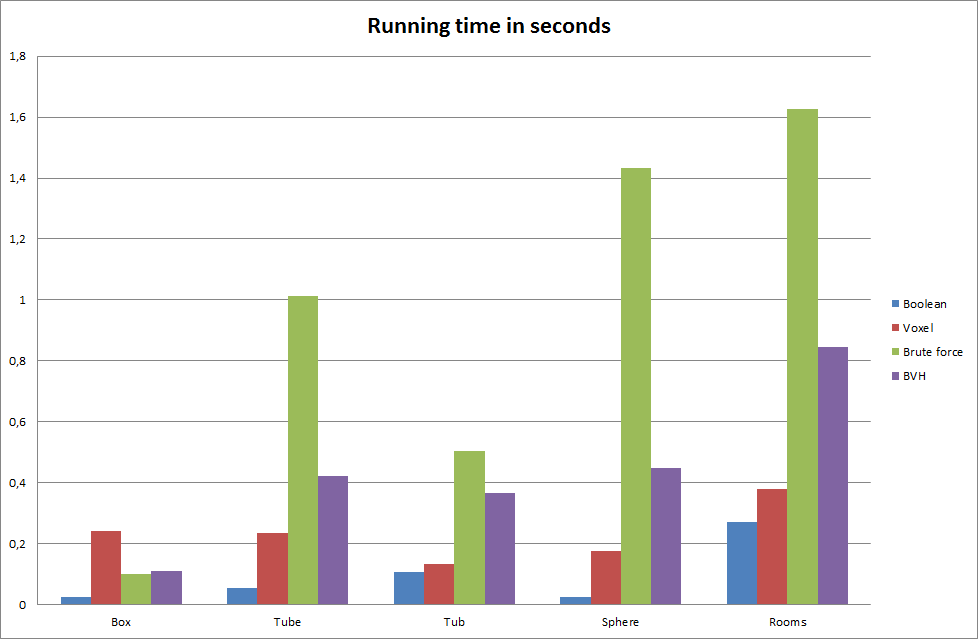
\includegraphics[width=\textwidth]{images/running_time_seconds}
                \caption{A gull}
                \label{fig:gull}
        \end{subfigure}%
        ~ %add desired spacing between images, e. g. ~, \quad, \qquad, \hfill etc.
          %(or a blank line to force the subfigure onto a new line)
        \begin{subfigure}[h]{0.3\textwidth}
%                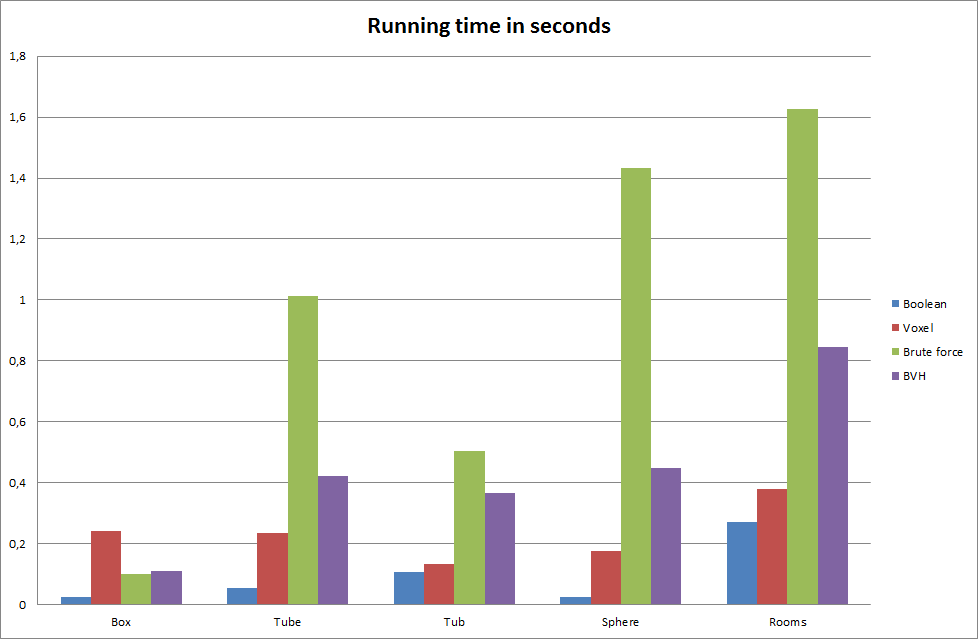
\includegraphics[width=\textwidth]{images/running_time_seconds}
                \caption{A tiger}
                \label{fig:tiger}
        \end{subfigure}
        \caption{Pictures of animals}\label{fig:animals}
\end{figure}


\begin{figure}[h]
    \centering
%    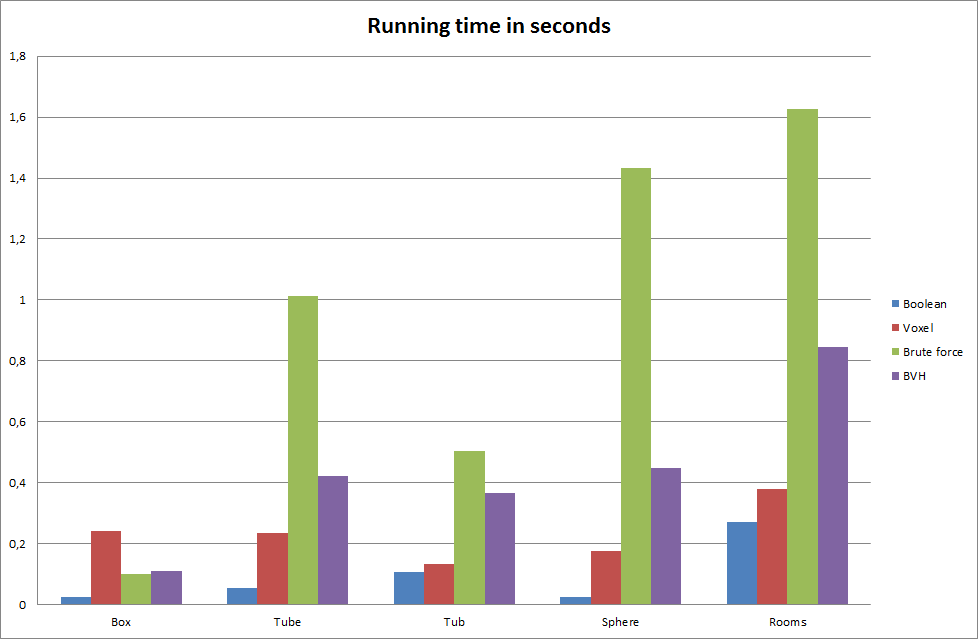
\includegraphics[width=0.45\linewidth]{images/running_time_seconds}
    \caption{Awesome Image}
    \label{fig:awesome_image1}
\end{figure}
\begin{figure}[h]
    \centering
%    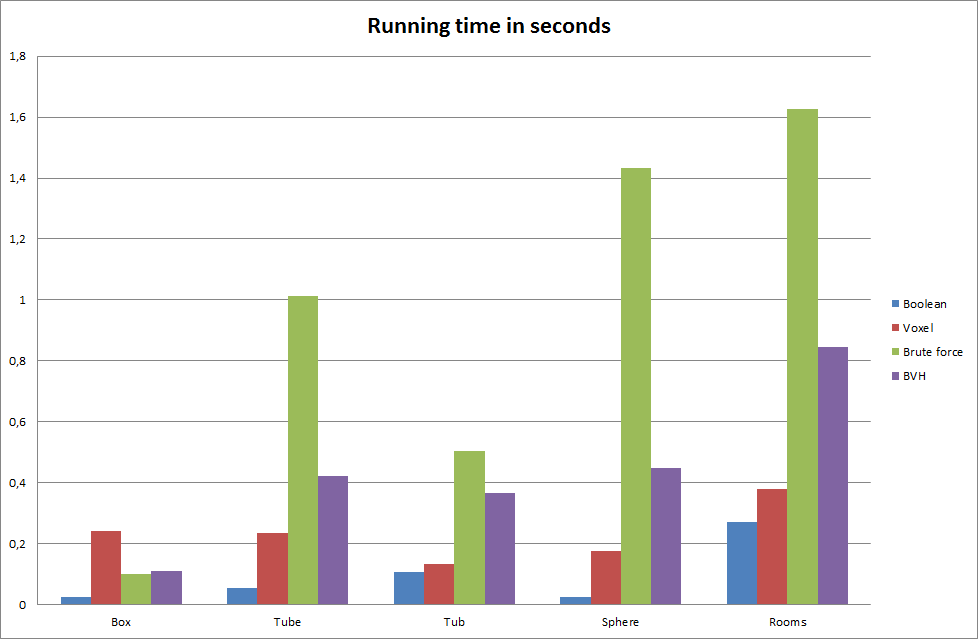
\includegraphics[width=0.45\textwidth]{images/running_time_seconds}
    \caption{Awesome Image}
    \label{fig:awesome_image2}
\end{figure}

This chapter will show the results. Figure~\ref{fig:awesome_image1} shows a photograph of a gull.

This \cite{wiki:123} cites wikipedia
\chapter{Discussion}

\chapter{Future Research and Conclusion}
This \cite{amanatides1987fast} sites something

\bibliographystyle{plain}
\bibliography{master}

\listoffigures
\listoftables
\appendix
\chapter{This is an appindex}
\section{First Appendix}
Hello world

\end{document}